\documentclass{sem5}
\institutename{Indian Institute of Information Technology, Vadodara}
\author{Hemant Kumar}
\idt{201352026}
%\team{teamname}
\collab{\textbf{Collaborator} - Dilip Puri(201351014)}

\coursename{Parallel Programming}
\ccode{\begin{small}CS403\end{small}}
\profname{Prof. Reshmi Mitra}

\type{Lab}
\typeid{05}
\submissiondate{\today}%dd/mm/yyyy
\deadline{Oct 03, 11:59 PM}%dd/mm/yyyy @hh:mm pm/am
\problemset{Helgrind (Thread Error Detector)}

\begin{document}
\begin{itemize}
\item[1] In the Helgrind tutorial link, familarize yourself with the use for: \\
\begin{enumerate}
\item Data race condition \\

 A data race occurs when multiple threads access a shared memory location with undetermined accessing order and at least one access is to write a new data into the shared memory location. 
In the program data race condition occurs when we want to increment same count with multiple threads. 


\item Ordering in POSIX locks \\

--track-lockorders=no|yes [default: yes] \\

When enabled (the default), Helgrind performs lock order consistency checking. For some buggy programs, the large number of lock order errors reported can become annoying, particularly if you're only interested in race errors. You may therefore find it helpful to disable lock order checking. 

\item POSIX misuses detection \\

there are many events when threads run on invalid time such as: \\
1. unlocking an invalid mutex \\
2. unlocking a not-locked mutex \\
3. unlocking a mutex held by a different thread \\ 
4. destroying an invalid or a locked mutex \\
5. recursively locking a non-recursive mutex\\

\end{enumerate}

\newpage
\item[2]- refer to the attached file\\
\section{verify the following}
\begin{enumerate}
\item  the put runs faster with 4 cores than 2 cores, but not 4 times as fast as a single core. \\

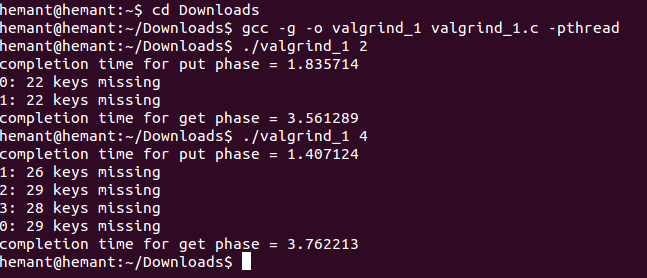
\includegraphics[scale=0.7]{result.png} \\
Output of fixed code\\
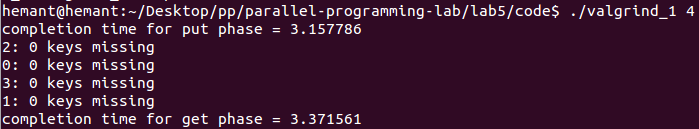
\includegraphics[scale=0.7]{fixed.png}\\
as we can see in the figure that is the result when the threads are run for 2 threads and 4 threads, the time taken on 4 threads is less but not the half of the time taken when 4 threads are used. 
this is happening when there occurs the data race condition as multiple threads tries to get the lock but the threads have to wait for the other thread to unlock the mutex lock. 
so more the threads more will be the race condition occurred.\\


\item  the get phase ran even slower \\

because of the more missing keys it took more time to get the access to the hash table and read the data. Also there were times when the mutex lock could not happen. Because of this mutex lock more conflicts are coming with the threads.
The application inserted 22+22 keys in phase 1 that phase 2 couldn't find.

\end{enumerate}

\section{Use Valgrind to find race condition. Using mutex lock to fix the race condition. Argue that your changes ensures correctness}

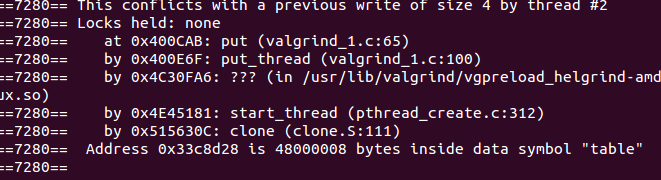
\includegraphics[scale=0.7]{helgring_output.png} \\


As we can see here that the two threads are conflicting to get the access to the table to put the data to the hash table but because there is is no ordering sequence that is causing no acces to both the threads.

 We can solve this problem by putting the lock for access before each thread that gets access to the table to update the data and then unlock the access for the other threads to get access.  


\begin{lstlisting}
put_thread(void *xa) 
{ 
	 assert(pthread_mutex_lock(&lock) == 0); 
  long n = (long) xa; 
  int i; 
  int b = NKEYS/nthread; 

  for (i = 0; i < b; i++) { 
    put(keys[b*n + i], n); 
  } 
    assert(pthread_mutex_unlock(&lock) == 0); 
}
\end{lstlisting}

Here we have taken mutex lock for the process that i have described above the figure.

\section{ Using “cachegrind” and “kcachegrind”, identify the most expensive function calls in terms of cycles spent. Instructions for the tools are available in Lab 4. Attach screen-shots whenever necessary.
}

\begin{enumerate}
\item cycles in the put function\\\\
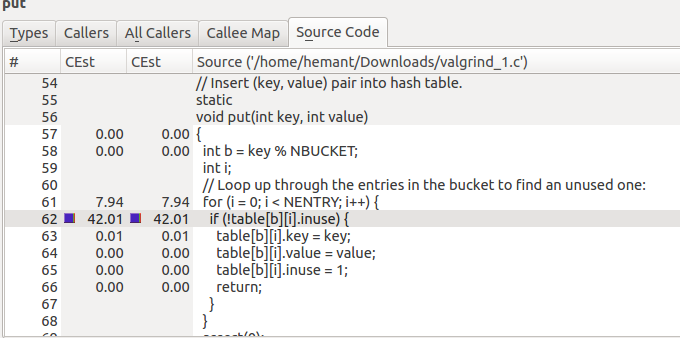
\includegraphics[scale=0.6]{cycles_in_put.png}\\
This is the screen shot showing that the if statement after the for loop is taking the maximum cycles as it has to check on every thread call whether the particular location is available or not to read the data.
\item cycles in the get function\\
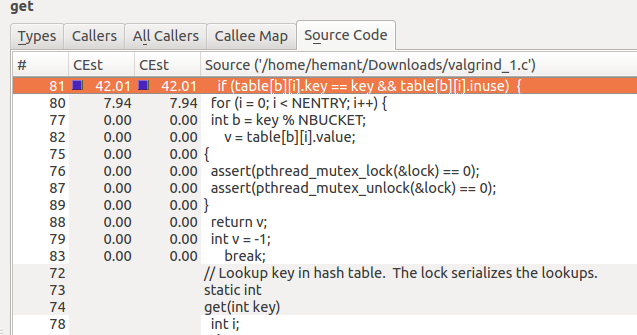
\includegraphics[scale=0.6]{cycles_in_get.png}

In put function also the if condition which is running after the for loop is taking the maximum cycles of the other functions.

But both the places are taking estimated cycles and are equal. So we can not distinguish between these positions. 

\end{enumerate}



\end{itemize}
\vspace{4cm}

\begin{center}
\textbf{Thank You}
\end{center}

\end{document}